\documentclass[a4paper,11pt]{article}
\usepackage[utf8x]{inputenc}
\usepackage{fullpage}
\usepackage[margin=1in]{geometry}
\usepackage{cite}
\usepackage{times}
\usepackage{setspace}
\usepackage{fancyhdr}
\usepackage{ifthen}
\usepackage{listings}
\usepackage[section]{placeins}
\usepackage{xtab}
\usepackage{url}

\usepackage{graphicx}
\usepackage{wrapfig}

\DeclareGraphicsExtensions{.pdf,.eps,.svg,.pgm}
\pagestyle{fancy}
\setboolean{@twoside}{false} 
    % EXTREMELY COMMON LaTeX PACKAGES TO INCLUDE:
    \usepackage{amsmath,amsthm, amsfonts,amssymb} % For AMS Beautification
    \usepackage{setspace} % For Single & Double Spacing Commands
    \usepackage[linktocpage,bookmarksopen,bookmarksnumbered,% For PDF navigation
		pdftitle={R21 Grant Proposal},%   and URL hyperlinks
		pdfauthor={Department of Electronic and Computing Systems},%
		pdfsubject={UC },%
		pdfkeywords={UC}]{hyperref}
           \usepackage{caption3} % load caption package kernel first
    \DeclareCaptionOption{parskip}[]{} % disable "parskip" caption option
    \usepackage[small]{caption}
\title{}
\author{}

\begin{document}

\begin{center}
\textbf{Section TITLE}\\
\end{center}
Body\cite{Carreira}.
\\
math and figure wrapping
\begin{wrapfigure}{l}{0.41\textwidth}
\[
    r_{ij}= 
\begin{cases}
    +1, & \text{with probability } {1 \over 6}\\
     0, & \text{with probability } {2 \over 3}\\
    -1, & \text{with probability } {1 \over 6}\\
\end{cases}
\]\caption*{ Approximate Random Projection Matrix\cite{Bingham}}
\end{wrapfigure}
\\
an image and wrapping possibly.
\begin{wrapfigure}{l}{0.45\textwidth}
\centering
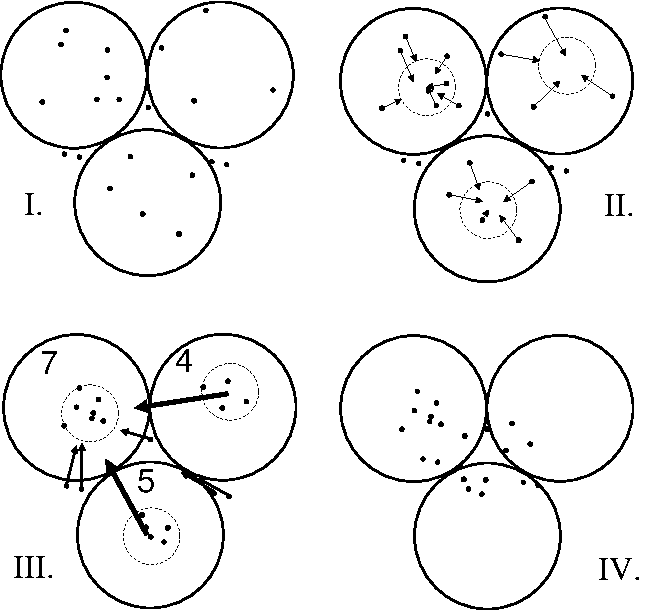
\includegraphics[scale=.6]{Diagram1.pdf}
\caption*{ \textbf{I.} Initial lattice assignment, \textbf{II.} Fine Grain
Iteration, \textbf{III.} Course Grain Iteration, \textbf{IV.} Updated Positions}
\end{wrapfigure}
and a blibliography

\bibliography{refs}
\bibliographystyle{ieeetr} \markright{ }

\end{document}
